\documentclass[a4paper, 12pt]{article}%тип документа

%отступы
\usepackage[left=2cm,right=2cm,top=2cm,bottom=3cm,bindingoffset=0cm]{geometry}
\setlength{\parindent}{5ex}

%Русский язык
\usepackage[T2A]{fontenc} %кодировка
\usepackage[utf8]{inputenc} %кодировка исходного кода
\usepackage[english,russian]{babel} %локализация и переносы

%Вставка картинок
\usepackage{graphicx}
\graphicspath{{pictures/}}
\DeclareGraphicsExtensions{.pdf,.png,.jpg}

%Графики
\usepackage{pgfplots}
\pgfplotsset{compat=1.9}

%Математика
\usepackage{amsmath, amsfonts, amssymb, amsthm, mathtools}

%Таблицы
\usepackage{longtable} 
\usepackage{float}

%Римские цифры
\newcommand{\RomanNumeralCaps}[1]{\uppercase\expandafter{\romannumeral#1}}

\usepackage{multirow}


\begin{document}
	\begin{titlepage}
		\begin{center}
			\textsc{Федеральное государственное автономное образовательное учреждение высшего образования«Московский физико-технический институт (национальный исследовательский университет)»\\[5mm]
			}
			
			\vfill
			
			\textbf{Отчёт по лабораторной работы 2.3.1\\[3mm]
				Современные средства
				получения и измерения вакуума.
				\\[50mm]
			}
			
		\end{center}
		
		\hfill
		\begin{minipage}{.5\textwidth}
			Выполнил студент:\\[2mm]
			Сериков Василий Романович\\[2mm]
			группа: Б03-102\\[5mm]
			
		\end{minipage}
		\vfill
		\begin{center}
			Москва, 2022 г.
		\end{center}
		
	\end{titlepage}
	
	\newpage
	\textbf{Аннотация}\\
	
	
	\textbf{Цель работы: }\\
	
	
	Изучить свойства и особенности вакуума при помощи экспериментального стенда выполненного на основе компактного высоковакуумного откачного поста Edwards серии EXPT с пластинчатороторным и турбомолекулярным насосами. Определить полный объем установки, высоковакуумной части, форвакуумной магистрали и насоса ТМН. Оцените эффективную скорость откачки системы форвакуумным насосом в области, где она почти постоянна. Оцените эффективную скорость откачки системы турбомолекулярным насосом в области, где она почти постоянна. Определите уровень течей по ухудшению вакуума после перекрытия откачки насосом ТМН.\\
	
	
	
	
	
	\textbf{Теоретические сведения: } \\
	
	
	В физике вакуумом называют состояние газа, при котором характерная длина свободного пробега молекул в газе $\lambda$ сравнима по порядку
	величины с характерным линейным размером сосуда $d$, в котором газ
	находится. Для воздуха при нормальных условиях $\lambda \approx 10^{-5}$ см, откуда
	видно, что воздух в жилых помещениях не находится в состоянии вакуума, но, например, внутри пористых материалов, таких как древесина, уже
	может находиться.
	
	
	Скорость откачки:
	\begin{equation}
		S = \frac{dV}{dt};
	\end{equation}	
	
	Падение давления:
	\begin{equation}
		\Delta P = P_{\text{вх}} - P_{\text{вых}};
	\end{equation}
	
	Пропускная способность:
	\begin{equation}
		U = \frac{Q}{\Delta P};
	\end{equation}
	
	Основное уравнение вакуумной механики:
	\begin{equation}
		\frac{1}{S_{0}} = \frac{1}{S_{text{н}}} + \frac{1}{U};
	\end{equation} 
	
	\begin{equation}
		Q_{\text{н}} = V\frac{P_{\text{к}} - P_{\text{н}}}{\Delta t}		
	\end{equation}
	
	Проводимость отверстия:
	\begin{equation}
		U_{\text{отв}} = \frac{1}{4} \pi R^{2} \sqrt{\frac{8kT}{\pi m}} \sim R^{2}\sqrt{T/m}
	\end{equation}
	
	Проводимость длинного трубопровода
	\begin{equation}
		U_{\text{тр}} = \frac{4}{3} \frac{R^{3}}{L} \sqrt{\frac{2\pi kT}{m}} \sim \frac{R^{3}}{L} \sqrt{\frac{T}{m}} 
	\end{equation}
	
	Уравнение откачки газа
	\begin{equation}
		P\left( t \right) = P_{1}\exp \left(- \frac{S_{0}}{V_{0}}t \right)
	\end{equation}
	
	
	Одна из основных характеристик систем, работающих при вакууме -- число Кнудсена:
	
	\begin{equation}
		Kn = \frac{\lambda}{d}, 
	\end{equation}
	
	$\lambda$ -- длина свободного пробега молекул газа, $d$ -- характерный размер системы.
	
	В зависимости от значений числа Кнудсена определяют:
	
	1) низкий вакуум -- $Kn \ll 1$
	
	2) средний вакуум -- $Kn \sim 1$
	
	3) высокий вакуум -- $Kn \gg 1$
	
	\textbf{Методика измерений: }\\
	
	\begin{figure}[h]
		\center{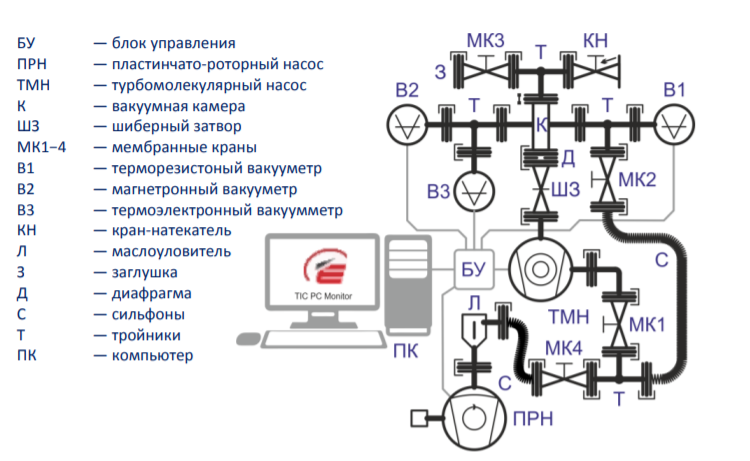
\includegraphics [scale=1]{Схема установки.png}}
		\caption {Схема экспериментальной установки}
	\end{figure}
	
	Экспериментальный стенд выполнен на основе компактного высоковакуумного откачного поста Edwards серии EXPT с пластинчатороторным и турбомолекулярным насосами, вакуумметров Edwards
	и вакуумных компонентов. Управление основными функциями откачного поста, контроль и запись параметров установки осуществляется блоком управления (БУ) через цифровой интерфейс RS-232
	с помощью специального программного обеспечения TIC PC Monitor10.
	Вакуумный пост Edwards EXPT (TY1211601) выполнен на базе
	пластинчато-роторного форвакуумного насоса Е2М1.5 (ПРН) и турбомолекулярного насоса EXPT 70H (ТМН). Откачка вакуумной камеры (К) может происходить как двумя насосами (ТМН и ДН) через шиберный затвор (ШЗ) и мембранные краны 1 и 4 (МК1, МК4), так и только форвакуумным насосом (ПРН) по схеме «байпас» (англ. bypass — обходной путь),
	выполненной на основе вакуумных компонентов: сильфонов (С), мембранных кранов 2 и 4 (МК2, МК4), тройников (Т), переходников.
	Для контроля и измерения давления в вакуумной камере используются цифровые вакууметры APG100-XM (В1) типа Пирани (терморезисторный), AIM-X (В2) инверсно-магнетронный и AIGX-S (В3) термоэлектронный (с накалённым катодом).
	Контролированный напуск воздушной атмосферы в камеру осуществляется через кран-натекатель LV10K (КН) с регулируемым потоком.
	Дополнительный выход с краном 3 (МК3) закрыт заглушкой (З) и служит
	для присоединения дополнительного объёма в случае необходимости.\\
	
	
	\textbf{Используемое оборудование: }\\
	
	Высоковакуумный откачной пост Edwards серии EXPT с пластинчатороторным и турбомолекулярным насосами, ПК, программа для записи показаний.\\
	
	
	\textbf{Результаты измерений и обработка данных: }\\
	
	\begin{enumerate}
	\item Определим объем камеры К по закону Бойля -- Мариотта: 
	$$ p_1(V_0 + V_k) = p_0 V_0 + p_{lim} V_k$$ где $p_0$ -- атмосферное давление, $p_1 = 2,49 \cdot 10^4$ Па, $V_0 = 252$ мл -- объем сильфона, $V_k$ -- объем камеры, $p_{lim} = 3,47 $ Па . Тогда $V_k$ = 760 мл.
	
	\item Определим объем форвакуумной магистрали: $$ p_2(V_0 + V_k + V_f) = p_1 (V_0 + V_k) + p_{lim} V_f$$ $V_f$ -- объем форвакуумной магистрали, $p_2 = 1,72 \cdot 10^4$ Па. Получим: $V_f$ = 453 мл.
	
	\item  Определим объем насоса:  $$ p_3(V_0 + V_k + V_f + V_{pomp}) = p_2 (V_0 + V_k + V_f) + p_{lim} V_{pomp}$$ $p_3 = 1,36\cdot 10^4$ Па, Получим: $V_{pomp}$ = 387 мл. 
	
	\item Тогда полный объем установки $V_{inst} = 1852$ мл.
	\item Погрешность измерения объемов: $\sigma_{V_k} = V_k \varepsilon_1$, где $\varepsilon_1 = 15\% $ -- точность измерения вакуумметра APG100-XM типа Пирани (В1), тогда $\sigma_{V_k} = \pm 114 $ Па, $\sigma_{V_f} = \pm 68 $ Па, $\sigma_{V_{pomp}} = \pm 58 $ Па, $\sigma_{V_inst} = \pm 144 $ Па.
	
	\item\textbf{ Оценим эффективную скорость откачки системы форвакуумным насосом в области, где она почти постоянна.}
	
	
	 Возьмем данные зависимости давления в камере К от времени откачки насосом.
	 По зависимости $\ln p$ от $t$ определим постоянную времени откачки $\tau$ в диапазоне давлений $p_1 = 10^0 - 10^2 = p_2$ мбар. Построим график зависимости $\ln p(t)$
	 $$ \tau = - \frac{t}{\ln p_1/p_2} => \tau = (22 \pm 1) c$$
	 
	 \newpage
	
	\begin{figure}[h]
		\center{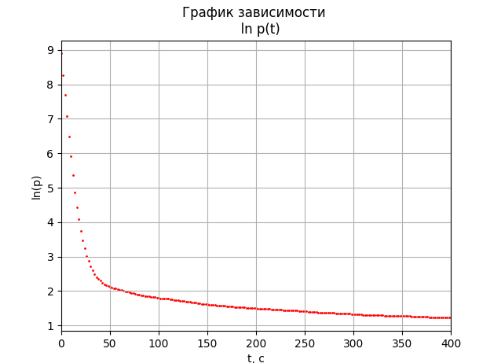
\includegraphics [scale=1]{FVN.png}}
	\end{figure}
	
	\item Рассчитаем эффективную скорость откачки $S_0$ и $S_{pomp}$
	$$ S_0 = \frac{V_k}{\tau} = (35 \pm 2) \text{ мл/с}$$
	$$ S_{pomp} = \frac{V_{pomp}}{\tau} = (81 \pm 2) \text{ мл/с}$$
	
	\item Определим суммарную пропускную способность $U$
	$$ U = \frac{S_{pomp} S_k}{S_{pomp} - S_0}  = (67 \pm 3) \text{ мл/с}$$
	
	\item \textbf{Оценим эффективную скорость откачки системы турбомолекулярным насосом в области, где она почти постоянна.}
	
	
	Аналогично п.6-8 определим те же параметры для ТМН.
	
	\item $\tau = (45 \pm 1) c$
	\item $S_0 = (17 \pm 2)  \text{ мл/с}$
	\item $ S_{pomp} = (40 \pm 2) \text{ мл/с}$
	\item $ U = (30 \pm 3) \text{ мл/с}$
	\newpage
	\begin{figure}[h]
		\center{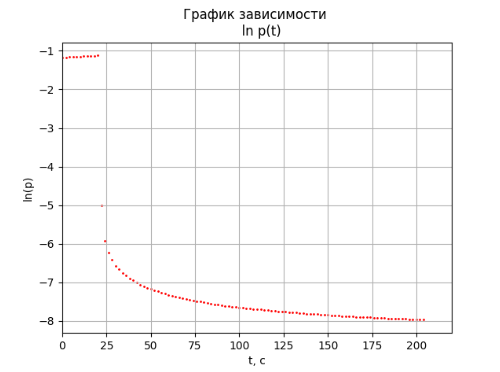
\includegraphics [scale=1]{TMN.png}}
	\end{figure}
	
	\item \textbf{Определим уровень течей по ухудшению вакуума после перекрытия откачки насосом ТМН.}
	
	
	$$ Q_n = V_k \frac{P' - P''}{\Delta t} = (7 \pm 1)\cdot 10^{-3} \text{л мбар/с,     где  } P' = 10^{-3}\text{мбар}, P'' = 10^{-5} \text{мбар}$$
	
	
	
	\begin{figure}[h]
		\center{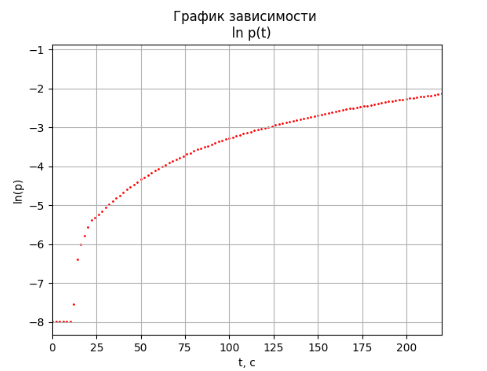
\includegraphics [scale=1]{flow.png}}
	\end{figure}
	
	
	\item \textbf{Оценим число Кнудсена для предельных давлений при форвакуумной и высоковакуумной откачке.}
	
	$$ Kn = \frac{\lambda}{d} = \frac{k_B T}{\sqrt 2 \pi \sigma^2 P V_k^{1/3}}, \text{где } \sigma = 0,3 \cdot 10^{-9} - \text{характерный диаметр молекулы воздуха}$$
	
	
	$Kn_{\text{ФН}} = 0,11 $\\
	
	
	$Kn_{\text{ТМН}} = 1143 $
	\end{enumerate}


	\textbf{Обсуждение результатов: }\\
	
	
	Проведя работу, мы определили с неплохой погрешностью объемы всех частей установки, построив графики зависимости $\ln p(t)$ мы смогли достаточно точно определить эффективные скорости откачки различными насосами. Полученное нами число Кнудсена для ФН и ТМН соответствуют теоретическому предположению.\\
	
	
	
	\textbf{Выводы: }\\
	
	
	В ходе работы мы научились пользоваться экспериментальным стендом выполненным на основе компактного высоковакуумного откачного поста Edwards серии EXPT с пластинчатороторным и турбомолекулярным насосами.Оценили эффективную скорость откачки системы форвакуумным  и турбомолекулярным насосами в области, где она почти постоянна.Определили уровень течей по ухудшению вакуума после перекрытия откачки насосом ТМН.Оценили число Кнудсена для предельных давлений при форвакуумной и высоковакуумной откачке.
	
	
	
\end{document}